\documentclass[tikz,border=0pt]{standalone}
\usepackage[american]{circuitikz}
\usetikzlibrary{arrows.meta,calc,positioning,decorations.pathmorphing,patterns}
\definecolor{zyloTeal}{HTML}{174A5B}
\definecolor{zyloTealTwo}{HTML}{246B7A}
\definecolor{zyloInk}{HTML}{1F2933}
\definecolor{zyloSoft}{HTML}{EAF4F4}
\definecolor{zyloPaper}{HTML}{F8FAFB}
\definecolor{zyloLine}{HTML}{44606B}
\definecolor{zyloOrange}{HTML}{D97706}
\begin{document}
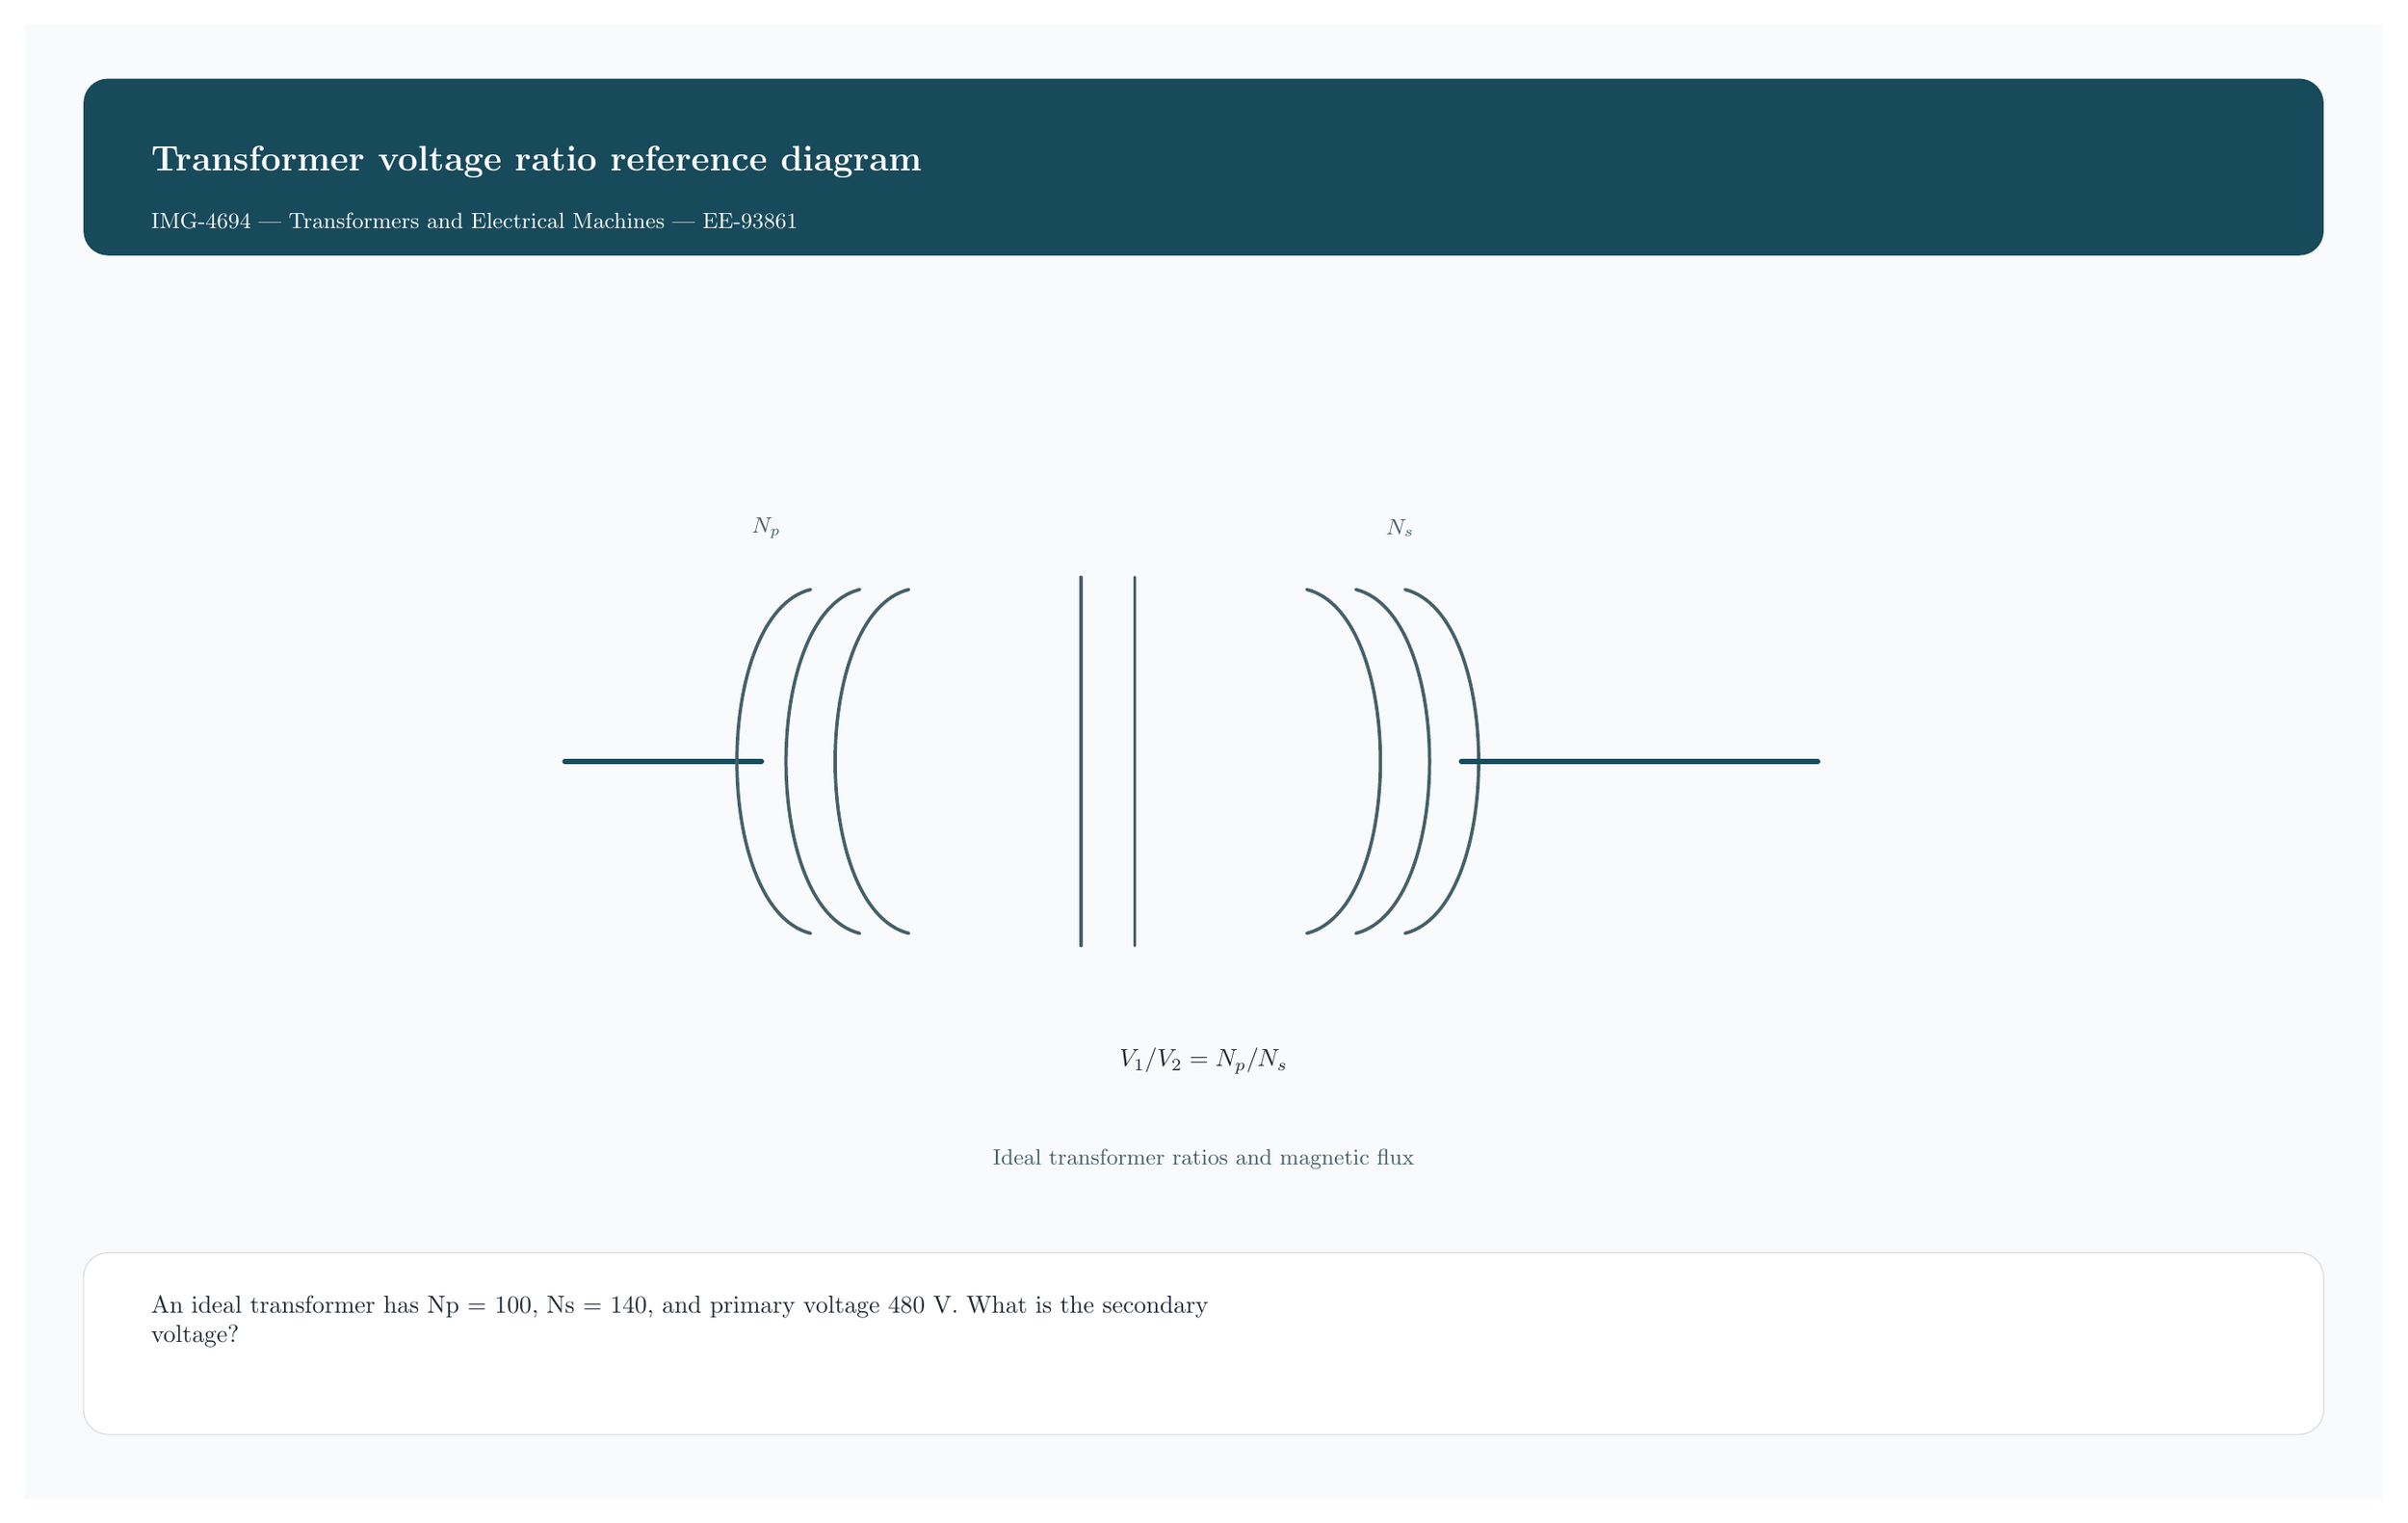
\begin{tikzpicture}[x=1pt,y=-1pt,>=Latex,line cap=round,line join=round]
\path[fill=zyloPaper] (0,0) rectangle (960,600);
\path[fill=zyloTeal,rounded corners=10pt] (24,22) rectangle (936,94);
\node[anchor=west,text=white,font=\bfseries\Large] at (48,56) {Transformer voltage ratio reference diagram};
\node[anchor=west,text=white!82,font=\small] at (48,80) {IMG-4694 | Transformers and Electrical Machines | EE-93861};
\tikzset{wire/.style={draw=zyloTeal,line width=2.2pt},thinwire/.style={draw=zyloLine,line width=1.35pt},accent/.style={draw=zyloOrange,line width=2.2pt},box/.style={draw=zyloTealTwo,fill=zyloSoft,line width=1.5pt,rounded corners=8pt}}
\draw[wire] (220,300) -- (300,300);
\draw[thinwire] (320,230) .. controls (280,240) and (280,360) .. (320,370);
\draw[thinwire] (340,230) .. controls (300,240) and (300,360) .. (340,370);
\draw[thinwire] (360,230) .. controls (320,240) and (320,360) .. (360,370);
\draw[thinwire] (430,225) -- (430,375); \draw[thinwire] (452,225) -- (452,375);
\draw[thinwire] (522,230) .. controls (562,240) and (562,360) .. (522,370);
\draw[thinwire] (542,230) .. controls (582,240) and (582,360) .. (542,370);
\draw[thinwire] (562,230) .. controls (602,240) and (602,360) .. (562,370);
\draw[wire] (585,300) -- (730,300);
\node[font=\small,text=zyloLine] at (302,205) {$N_p$}; \node[font=\small,text=zyloLine] at (560,205) {$N_s$};
\node[text=zyloInk] at (480,422) {$V_1/V_2=N_p/N_s$};
\node[font=\small,text=zyloLine] at (480,462) {Ideal transformer ratios and magnetic flux};
\path[draw=black!15,fill=white,rounded corners=10pt] (24,500) rectangle (936,574);
\node[anchor=west,text width=860pt,align=left,text=zyloInk,font=\normalsize] at (48,528) {An ideal transformer has Np = 100, Ns = 140, and primary voltage 480 V. What is the secondary\\voltage?};
\end{tikzpicture}
\end{document}
